\section{講義概要}


\begin{frame}
\frametitle{今日の内容}



\begin{enumerate}
\item 三角関数, 指数関数, 対数関数の微分,
\end{enumerate} 



\end{frame}





%%%%%%%%%%%%%%%%%%%%%%%%%%%%%%%%%%%%%%%%%%%%%%%%%%%%%%%%%%%%%%%%%%%%%%%%%%%%%%%%%%%%%%%
%%%%%%%%%%%%%%%%%%%%%%%%%%%%%%%%%%%%%%%%%%%%%%%%%%%%%%%%%%%%%%%%%%%%%%%%%%%%%%%%%%%%%%%

\section{三角関数の微分}

\begin{frame}
\frametitle{三角関数の微分}


\vspace{-4mm}

三角関数の微分を議論するために必要な準備を行う. 

\vspace{-1mm}

\begin{Thm} \label{準備}
\begin{enumerate}
\item $\displaystyle\lim_{x \to 0} \frac{\sin x}{x}=1$, 
\item  $\displaystyle \lim_{x \to 0} \frac{1-\cos x}{x}=0$. 
\end{enumerate}
\end{Thm}
弧度法において, $x$が弧の長さであることから$0<x<\pi/2$において次の不等式が成立する. 
(扇形と底辺を共有する2つの三角形の面積を比較しても良い.)
\vspace{-6mm}

 \begin{figure}[htbp]
 \begin{center} 
  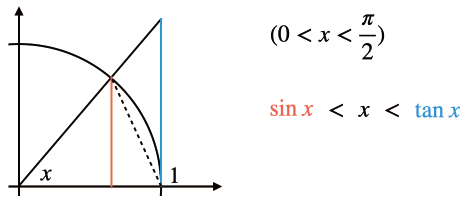
\includegraphics[width=65mm]{calculus5/sintan.png}
 \end{center}
\end{figure}

\vspace{-10mm}

\end{frame}





%%%%%%%%%%%%%%%%%%%%%%%%%%%%%%%%%%%%%%%%%%%%%%%%%%%%%%%%%%%%%%%%%%%%%%%%%%%%%%%%%%%%%%%
%%%%%%%%%%%%%%%%%%%%%%%%%%%%%%%%%%%%%%%%%%%%%%%%%%%%%%%%%%%%%%%%%%%%%%%%%%%%%%%%%%%%%%%


\begin{frame}
\frametitle{定理\ref{準備}\ctext{1}の証明}

$0<x<\pi/2$において
\begin{itemize}
\item $\sin x < x$より, $\frac{\sin x}{x}<1$. 
\item $x < \tan x=\frac{\sin x}{\cos x}$より, $\cos x < \frac{\sin x}{x}$.   
\end{itemize}
纏めると
$$
\cos x < \frac{\sin x}{x} < 1. 
$$
$x \to +0$なる極限をとると
$$
\lim_{x \to +0} \cos x \le \lim_{x \to +0} \frac{\sin x}{x} \le \lim_{x \to +0} 1. 
$$
これより, $\displaystyle\lim_{x \to +0} \frac{\sin x}{x}=1$. (挟み撃ちの定理)\\
\ \\

同様の議論で左極限も$\displaystyle\lim_{x \to -0} \frac{\sin x}{x}=1$.  

\end{frame}



%%%%%%%%%%%%%%%%%%%%%%%%%%%%%%%%%%%%%%%%%%%%%%%%%%%%%%%%%%%%%%%%%%%%%%%%%%%%%%%%%%%%%%%
%%%%%%%%%%%%%%%%%%%%%%%%%%%%%%%%%%%%%%%%%%%%%%%%%%%%%%%%%%%%%%%%%%%%%%%%%%%%%%%%%%%%%%%


\begin{frame}
\frametitle{定理\ref{準備}\ctext{2}の証明}

$\sin^2x +\cos^2 x=1$より
$$
\frac{1-\cos x}{x}
=
\frac{1-\cos ^2x}{x(1+\cos x)}
=
\frac{\sin ^2x}{x(1+\cos x)}
=
\frac{\sin x}{x}
\frac{\sin x}{1+\cos x}
$$
であるから 
$$
\lim_{x \to 0} \frac{1-\cos x}{x}=
\lim_{x \to 0} (\frac{\sin x}{x}
\frac{\sin x}{1+\cos x})
=1 \cdot \frac{0}{1+1}=0. 
$$

\end{frame}




%%%%%%%%%%%%%%%%%%%%%%%%%%%%%%%%%%%%%%%%%%%%%%%%%%%%%%%%%%%%%%%%%%%%%%%%%%%%%%%%%%%%%%%
%%%%%%%%%%%%%%%%%%%%%%%%%%%%%%%%%%%%%%%%%%%%%%%%%%%%%%%%%%%%%%%%%%%%%%%%%%%%%%%%%%%%%%%


\begin{frame}
\frametitle{三角関数の微分}



\begin{Thm} \label{三角関数微分}
\begin{enumerate}
\item $(\sin x)'=\cos x$,
\item  $(\cos x)' = -\sin x$,
\item $(\tan x)'=\frac{1}{\cos^2 x}$. 
\end{enumerate}
\end{Thm}

三角関数の加法定理を思い出しておく. 
\begin{itemize}
\item $\sin(\alpha+\beta)=\sin \alpha \cos \beta + \cos \alpha \sin \beta$
\item $\cos(\alpha+\beta)=\cos \alpha \cos \beta - \sin \alpha \sin \beta$
\end{itemize}

\end{frame}
\begin{slide}{加法定理の図的な説明}
%\begin{eqnarray}
%\sin(A+B) &=& \sin{A}\cos{B} + \sin{B}\cos{A} \\
%\sin(A-B) &=& \sin{A}\cos{B} - \sin{B}\cos{A} \\
%\cos(A+B) &=& \cos{A}\cos{B}-\sin{A}\sin{B} \\
%\cos(A-B)&=&\cos{A}\cos{B}+\sin{A}\sin{B}
%\end{eqnarray}
\begin{figure}[h]                                                                      
\centering
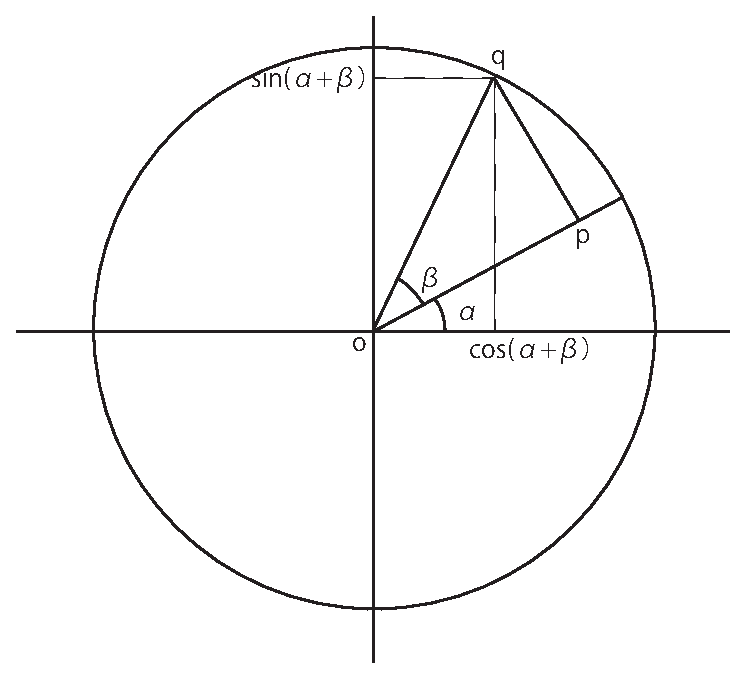
\includegraphics[width=3cm]{calculus5/add.eps}
%\caption{加法定理の図解}
%\label{fig:additive}
\end{figure}
\begin{equation}
\overrightarrow{op} = \cos{\beta}(\cos{\alpha}, \sin{\alpha})
\end{equation}
であり、$\overrightarrow{pq}$は$\overrightarrow{op}$に直交して長さが$\sin{\beta}$であるため
\begin{equation}
\overrightarrow{pq} = \sin{\beta}(-\sin{\alpha}, \cos{\alpha})
\end{equation}
となるため$\overrightarrow{oq}$は
\begin{eqnarray}
\overrightarrow{oq} &=& \overrightarrow{op}+\overrightarrow{pq}\nonumber \\
&=& (\cos{\alpha}\cos{\beta} - \sin{\alpha}\sin{\beta}, \sin{\alpha}\cos{\beta}+\sin{\beta}\cos{\alpha})
\end{eqnarray}
となり、加法定理を与える。
\end{slide}


%%%%%%%%%%%%%%%%%%%%%%%%%%%%%%%%%%%%%%%%%%%%%%%%%%%%%%%%%%%%%%%%%%%%%%%%%%%%%%%%%%%%%%%
%%%%%%%%%%%%%%%%%%%%%%%%%%%%%%%%%%%%%%%%%%%%%%%%%%%%%%%%%%%%%%%%%%%%%%%%%%%%%%%%%%%%%%%


\begin{frame}
\frametitle{定理\ref{三角関数微分}\ctext{1}の証明}

加法定理より
\begin{align*}
\sin(x +h)-\sin x & = \sin x \cos h + \cos x \sin h -\sin x \\
& =  \cos x \sin h + \sin x( \cos h-1)
\end{align*}
であるから
\begin{align*}
(\sin x)' &= \lim_{h \to 0} \frac{\sin(x +h)-\sin x}{h} \\
& =  \lim_{h \to 0} (\cos x \frac{\sin h}{h} + \sin x \frac{\cos h-1}{h}) \\
& =\cos x \cdot 1 + \sin x \cdot 0 \\
& = \cos x. 
\end{align*}
\end{frame}


%%%%%%%%%%%%%%%%%%%%%%%%%%%%%%%%%%%%%%%%%%%%%%%%%%%%%%%%%%%%%%%%%%%%%%%%%%%%%%%%%%%%%%%
%%%%%%%%%%%%%%%%%%%%%%%%%%%%%%%%%%%%%%%%%%%%%%%%%%%%%%%%%%%%%%%%%%%%%%%%%%%%%%%%%%%%%%%


\begin{frame}
\frametitle{定理\ref{三角関数微分}\ctext{2}の証明}

加法定理より
\begin{align*} 
\cos(x +h)-\cos x & = \cos x \cos h - \sin x \sin h -\cos x \\
& =  \cos x (\cos h-1) - \sin x \sin h
\end{align*}
であるから
\begin{align*}
(\cos x)' &= \lim_{h \to 0} \frac{\cos(x +h)-\cos x}{h} \\
& =  \lim_{h \to 0} (\cos x \frac{\cos h-1}{h} - \sin x \frac{\sin h}{h}) \\
& =\cos x \cdot 0 - \sin x \cdot 1 \\
& = -\sin x. 
\end{align*}
\end{frame}


%%%%%%%%%%%%%%%%%%%%%%%%%%%%%%%%%%%%%%%%%%%%%%%%%%%%%%%%%%%%%%%%%%%%%%%%%%%%%%%%%%%%%%%
%%%%%%%%%%%%%%%%%%%%%%%%%%%%%%%%%%%%%%%%%%%%%%%%%%%%%%%%%%%%%%%%%%%%%%%%%%%%%%%%%%%%%%%


\begin{frame}
\frametitle{定理\ref{三角関数微分}\ctext{3}の証明}

商の微分公式より
\begin{align*} 
(\tan x)' &= \Big( \frac{\sin x}{\cos x} \Big)' \\
&= \frac{(\sin x)'\cos x - \sin x (\cos x)'}{\cos^2 x} \\
&= \frac{\cos^2 x + \sin^2 x}{\cos^2 x} \\
&= \frac{1}{\cos^2 x}. 
\end{align*}

\end{frame}


%%%%%%%%%%%%%%%%%%%%%%%%%%%%%%%%%%%%%%%%%%%%%%%%%%%%%%%%%%%%%%%%%%%%%%%%%%%%%%%%%%%%%%%
%%%%%%%%%%%%%%%%%%%%%%%%%%%%%%%%%%%%%%%%%%%%%%%%%%%%%%%%%%%%%%%%%%%%%%%%%%%%%%%%%%%%%%%


\begin{frame}
\frametitle{三角関数の微分}

\begin{Prob}
次の関数の導関数を求めよ. 
\begin{enumerate}
\item $\sin^2 x$
\item $\sin^3 x$
\item $\sin x \cos x$
\item $\frac{\cos x}{x}$
\end{enumerate}
\end{Prob}

\end{frame}


%%%%%%%%%%%%%%%%%%%%%%%%%%%%%%%%%%%%%%%%%%%%%%%%%%%%%%%%%%%%%%%%%%%%%%%%%%%%%%%%%%%%%%%
%%%%%%%%%%%%%%%%%%%%%%%%%%%%%%%%%%%%%%%%%%%%%%%%%%%%%%%%%%%%%%%%%%%%%%%%%%%%%%%%%%%%%%%

\section{指数関数と対数関数の微分}

\begin{frame}
\frametitle{ネイピア数}

ネイピア数$e=2.71828\dots$に関して, 次が成立する.  
$$
e=\lim_{x \to +\infty} \Big(1+\frac{1}{x}\Big)^x = \lim_{x \to -\infty} \Big(1+\frac{1}{x}\Big)^x. 
$$
これは$\displaystyle e=\lim_{x\to 0}(1+x)^\frac{1}{x}$とも同値である. \\
\ \\

いくつか計算してみると
\begin{align*}
(1+\frac{1}{10})^{10}&=2.5937\dots, \ \ \ 
(1+\frac{1}{100})^{100}=2.7048\dots, \\
(1+\frac{1}{1000})^{1000}&=2.7169\dots, \ \ \ 
(1+\frac{1}{10000})^{10000}=2.7181\dots, 
\end{align*}

\end{frame}




%%%%%%%%%%%%%%%%%%%%%%%%%%%%%%%%%%%%%%%%%%%%%%%%%%%%%%%%%%%%%%%%%%%%%%%%%%%%%%%%%%%%%%%
%%%%%%%%%%%%%%%%%%%%%%%%%%%%%%%%%%%%%%%%%%%%%%%%%%%%%%%%%%%%%%%%%%%%%%%%%%%%%%%%%%%%%%%



\begin{frame}
\frametitle{準備}

指数関数と対数関数の微分を議論するために必要な準備を行う. 

\begin{Thm} \label{準備2}
\begin{enumerate}
\item $\displaystyle \lim_{h \to 0} \frac{e^h-1}{h}=1$, 
\item  $\displaystyle \lim_{h \to 0} \frac{\log(1+h)}{h}=1$. 
\end{enumerate}
\end{Thm}


\end{frame}



%%%%%%%%%%%%%%%%%%%%%%%%%%%%%%%%%%%%%%%%%%%%%%%%%%%%%%%%%%%%%%%%%%%%%%%%%%%%%%%%%%%%%%%
%%%%%%%%%%%%%%%%%%%%%%%%%%%%%%%%%%%%%%%%%%%%%%%%%%%%%%%%%%%%%%%%%%%%%%%%%%%%%%%%%%%%%%%


\begin{frame}
\frametitle{定理\ref{準備2}の証明}

まず\ctext{2}を示す. 
\begin{align*} 
\lim_{h \to 0} \frac{\log(1+h)}{h} & = \lim_{h \to 0} \log(1+h)^{\frac{1}{h}} \\
& = \log \big( \lim_{h \to 0} (1+h)^{\frac{1}{h}} \big) \ \ \ (\text{対数関数の連続性})\\
& = \log e = 1. 
\end{align*}
次に\ctext{1}を示す. 
まず$t=e^h-1$とおくと, $h\to 0$のとき$t\to0$である. 
また$e^h=1+t$より$h=\log (1+t)$であるから, \ctext{2}より
$$
\lim_{h \to 0} \frac{e^h-1}{h}=\lim_{t \to 0} \frac{t}{\log(1+t)}=1. 
$$

\end{frame}


%%%%%%%%%%%%%%%%%%%%%%%%%%%%%%%%%%%%%%%%%%%%%%%%%%%%%%%%%%%%%%%%%%%%%%%%%%%%%%%%%%%%%%%
%%%%%%%%%%%%%%%%%%%%%%%%%%%%%%%%%%%%%%%%%%%%%%%%%%%%%%%%%%%%%%%%%%%%%%%%%%%%%%%%%%%%%%%


\begin{frame}
\frametitle{指数関数の微分}

 指数関数$e^x$は微分しても不変であるという特殊な性質を持つ. 

\begin{Thm} 
$$(e^x)'=e^x$$
\end{Thm}

定理\ref{準備2}\ctext{1}より
\begin{align*} 
(e^x)' &= \lim_{h\to0}\frac{e^{x+h}-e^x}{h}=\lim_{h\to0}e^x \frac{e^h-1}{h}=e^x\cdot 1 = e^x. 
\end{align*}

微分して不変な関数は$e^x$の定数倍しかないことも知られている. 
つまり微分方程式$f'(x)=f(x)$の解は$f(x)=Ce^x$の形($C$:定数). 
底が$e$でない場合は講義の後半で扱う. 

\end{frame}



%%%%%%%%%%%%%%%%%%%%%%%%%%%%%%%%%%%%%%%%%%%%%%%%%%%%%%%%%%%%%%%%%%%%%%%%%%%%%%%%%%%%%%%
%%%%%%%%%%%%%%%%%%%%%%%%%%%%%%%%%%%%%%%%%%%%%%%%%%%%%%%%%%%%%%%%%%%%%%%%%%%%%%%%%%%%%%%


\begin{frame}
\frametitle{対数関数の微分}


\begin{Thm} 
$$(\log x)'=\frac{1}{x}$$
\end{Thm}

定理\ref{準備2}\ctext{2}より \vspace{-2mm}
\begin{align*} 
(\log x)' &= \lim_{h\to0}\frac{\log(x+h)-\log x}{h} \\
&= \lim_{h\to0}\frac{1}{h} \log \frac{x+h}{x} = \lim_{h\to0}\frac{1}{h} \log (1+\frac{h}{x}) \\
&= \lim_{t\to0}\frac{1}{tx} \log (1+t) = \lim_{t\to0}\frac{1}{x} \frac{\log (1+t)}{t} \\
&=\frac{1}{x}\cdot 1=\frac{1}{x}. 
\end{align*}

途中で$t=\frac{h}{x}$なる変数変換をしている. 

\end{frame}



%%%%%%%%%%%%%%%%%%%%%%%%%%%%%%%%%%%%%%%%%%%%%%%%%%%%%%%%%%%%%%%%%%%%%%%%%%%%%%%%%%%%%%%
%%%%%%%%%%%%%%%%%%%%%%%%%%%%%%%%%%%%%%%%%%%%%%%%%%%%%%%%%%%%%%%%%%%%%%%%%%%%%%%%%%%%%%%




%%%%%%%%%%%%%%%%%%%%%%%%%%%%%%%%%%%%%%%%%%%%%%%%%%%%%%%%%%%%%%%%%%%%%%%%%%%%%%%%%%%%%%%
%%%%%%%%%%%%%%%%%%%%%%%%%%%%%%%%%%%%%%%%%%%%%%%%%%%%%%%%%%%%%%%%%%%%%%%%%%%%%%%%%%%%%%%



\section{一般の指数関数の微分}


\begin{frame}
\frametitle{一般の指数関数の微分}


\begin{Thm} 
$a>0$に関して
$$(a^x)'=a^x \log a$$
\end{Thm}

$a=e^{\log a}$に注意すると
$$
a^x=(e^{\log a})^x=e^{x \log a}
$$
であるから, 
$f(y)=e^y$と$g(x)=x \log a$を用いて$f(g(x))=a^x=e^{x \log a}$と書けることから
\begin{align*} 
(a^x)' &= (e^y)'  =e^y \cdot y' =a^x \log a. 
\end{align*}


\end{frame}


%%%%%%%%%%%%%%%%%%%%%%%%%%%%%%%%%%%%%%%%%%%%%%%%%%%%%%%%%%%%%%%%%%%%%%%%%%%%%%%%%%%%%%%
%%%%%%%%%%%%%%%%%%%%%%%%%%%%%%%%%%%%%%%%%%%%%%%%%%%%%%%%%%%%%%%%%%%%%%%%%%%%%%%%%%%%%%%


\section{対数関数の微分の拡張}

\begin{frame}
\frametitle{対数関数の微分の拡張}

$\log x$の定義域は$x>0$であるが, $\log |x|$を考えることで, 定義域を$x\neq 0$なる実数全体に拡張される. 

 \begin{figure}[htbp]
 \begin{center} 
  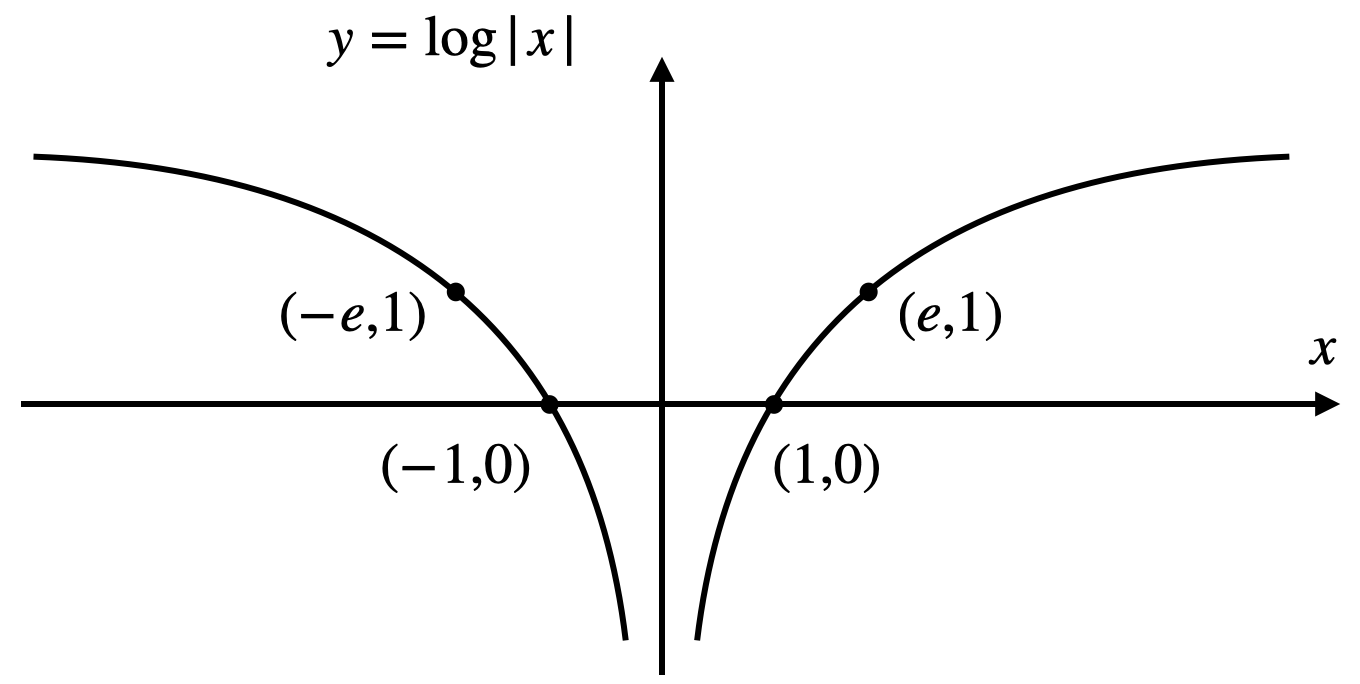
\includegraphics[width=90mm]{calculus5/log_abs.png}
 \end{center}
\end{figure}


\end{frame}


%%%%%%%%%%%%%%%%%%%%%%%%%%%%%%%%%%%%%%%%%%%%%%%%%%%%%%%%%%%%%%%%%%%%%%%%%%%%%%%%%%%%%%%
%%%%%%%%%%%%%%%%%%%%%%%%%%%%%%%%%%%%%%%%%%%%%%%%%%%%%%%%%%%%%%%%%%%%%%%%%%%%%%%%%%%%%%%


\begin{frame}
\frametitle{対数関数の微分の拡張}


\begin{Thm} 
$$(\log |x|)'=\frac{1}{x}$$
\end{Thm}

\begin{itemize}
\item $x>0$の場合
$$
(\log |x|)' = (\log x)'=\frac{1}{x}
$$
\item $x<0$の場合
$$
(\log |x|)' = (\log (-x))'=\frac{1}{-x} \cdot (-1)=\frac{1}{x}. 
$$
\end{itemize}


\end{frame}


%%%%%%%%%%%%%%%%%%%%%%%%%%%%%%%%%%%%%%%%%%%%%%%%%%%%%%%%%%%%%%%%%%%%%%%%%%%%%%%%%%%%%%%
%%%%%%%%%%%%%%%%%%%%%%%%%%%%%%%%%%%%%%%%%%%%%%%%%%%%%%%%%%%%%%%%%%%%%%%%%%%%%%%%%%%%%%%


\section{対数微分}

\begin{frame}
\frametitle{対数微分}



\begin{Thm} \label{対数微分}
微分可能な関数$g(x)$に対して
$$(\log |g(x)|)'=\frac{g'(x)}{g(x)}$$
\end{Thm}

$f(y)=\log |y|$と$g(x)$を用いて$f(g(x))=\log|g(x)|$と書けることから
$$
(\log |g(x)|)'=\frac{1}{g(x)}\cdot g'(x)=\frac{g'(x)}{g(x)}. 
$$
関数の対数を取ってから微分する方法は\underline{対数微分}と呼ばれ, 様々な場面に現れる. 

\end{frame}


%%%%%%%%%%%%%%%%%%%%%%%%%%%%%%%%%%%%%%%%%%%%%%%%%%%%%%%%%%%%%%%%%%%%%%%%%%%%%%%%%%%%%%%
%%%%%%%%%%%%%%%%%%%%%%%%%%%%%%%%%%%%%%%%%%%%%%%%%%%%%%%%%%%%%%%%%%%%%%%%%%%%%%%%%%%%%%%


\begin{frame}
\frametitle{$(x^a)'=ax^{a-1}$}



\begin{Thm} 
$a \in \R$に関して, $x>0$において
$$
(x^a)'=ax^{a-1}.
$$
\end{Thm}
$g(x)=x^a$とすれば
$$
(\log |g(x)|)'= (\log x^a)'= (a \log x)'=\frac{a}{x}. 
$$
定理\ref{対数微分}より
$$
\frac{a}{x}=\frac{g'(x)}{g(x)}=\frac{(x^a)'}{x^a}
$$
であるから
$$
(x^a)'=a x^{a-1}. 
$$
これは対数微分の典型的な応用例. 

\end{frame}


%%%%%%%%%%%%%%%%%%%%%%%%%%%%%%%%%%%%%%%%%%%%%%%%%%%%%%%%%%%%%%%%%%%%%%%%%%%%%%%%%%%%%%%
%%%%%%%%%%%%%%%%%%%%%%%%%%%%%%%%%%%%%%%%%%%%%%%%%%%%%%%%%%%%%%%%%%%%%%%%%%%%%%%%%%%%%%%


\begin{frame}
\frametitle{$(x^a)'=ax^{a-1}$}


具体的に計算すれば
\begin{align*}
(\sqrt{x})' &= (x^{\frac{1}{2}})'=\frac{1}{2}x^{-\frac{1}{2}}= \frac{1}{2 \sqrt{x}}, \\
(\sqrt[3]{x^2})' &= (x^{\frac{2}{3}})'=\frac{2}{3}x^{-\frac{1}{3}}= \frac{2}{3 \sqrt[3]{x}}
\end{align*}

% x^xも対数微分の良い応用例

\end{frame}



%%%%%%%%%%%%%%%%%%%%%%%%%%%%%%%%%%%%%%%%%%%%%%%%%%%%%%%%%%%%%%%%%%%%%%%%%%%%%%%%%%%%%%%
%%%%%%%%%%%%%%%%%%%%%%%%%%%%%%%%%%%%%%%%%%%%%%%%%%%%%%%%%%%%%%%%%%%%%%%%%%%%%%%%%%%%%%%


\begin{slide}{一般化二項分布}
$a$を実数とした時、
\begin{equation}
f(x) = (1+x)^{\alpha} \nonumber
\end{equation}
は以下の無限級数と同値である。
\begin{equation}
f(x) = (1+x)^{\alpha} = \sum_{k=0}^\infty \binom{\alpha}{k}x^k \label{eq:gb}
\end{equation}
ここで以下を用いている。
\begin{equation}
\binom{\alpha}{k} = \frac{\alpha(\alpha - 1)(\alpha - 2) \cdots (\alpha - k + 1)}{k!} 
\end{equation}
\rref{eq:gb}はべき級数なので、微分できて以下となる。
\begin{equation}
f'(x) = \alpha + \alpha(\alpha - 1) x + \frac{\alpha(\alpha -1 )(\alpha -2)}{2}x^2+\cdots 
\end{equation}
これにより以下が成立する。
\begin{equation}
(1 + x) f'(x) = \alpha f(x) \label{eq:gbcore}
\end{equation}
\end{slide}
\begin{slide}{一般化二項分布 2}
ここで
\begin{equation}
\left((1+x)^{-\alpha} f(x)\right)' = -\alpha(1+x)^{-\alpha -1} f(x) + (1+x)^{-\alpha} f'(x)
\end{equation}
なので、\rref{eq:gbcore}を代入して
\begin{equation}
\left((1+x)^{-\alpha} f(x)\right)' = -\alpha(1+x)^{-\alpha -1} f(x) + (1+x)^{-\alpha-1} f(x) = 0
\end{equation}
微分してゼロになる関数は定数であるため、
\begin{equation}
\left((1+x)^{-\alpha} f(x)\right) = C
\end{equation}
であり
\begin{equation}
f(x) = C(1+x)^{\alpha}
\end{equation}
\end{slide}

\section{今日のまとめ}
\begin{frame}
\frametitle{まとめ}   


\begin{enumerate}
\item 三角関数, 指数関数, 対数関数の微分,
\end{enumerate} 


\end{frame}
